\chapter{基因工程与生物技术}\label{ch:b3:genetic-engineering}

直到 1982 年，世界上每一位糖尿病患者
都靠从猪和牛胰腺中提取的胰岛素维持生命——
制取一千克激素，约需八千千克腺体——
并有一部分患者会对这种外源蛋白产生免疫反应。
同年，首个由基因工程生物制成的药物上市：
人胰岛素，由携带人类基因（位于\omterm{def:b3:genetic-engineering:tools}{质粒}上）的
\emph{Escherichia coli} 合成。
使之成为可能的工具，是在前十年间逐步建立起来的——
能在特定序列处切割 DNA 的酶，把片段连接起来的酶，
以及把 DNA 带入细胞并在其中复制的\omterm{def:b3:genetic-engineering:tools}{质粒}。
随后几十年间，又加入了\omterm{def:b3:genetic-engineering:pcr}{聚合酶链反应}、向胚胎中注射基因，
以及自 2012 年起，被改造成可编程“剪刀”的细菌免疫系统——
它能在活细胞中改写基因组中的一个碱基。
本章讲述这些工具、支配其使用的算术，
以及借助它们所构建的成果，
从发光的小鼠到镰状细胞病的治疗。

\section{切割、连接与复制 DNA}

\begin{definition}[限制酶、DNA 连接酶与载体]\label{def:b3:genetic-engineering:tools}
\index{限制酶}\index{黏性末端}\index{DNA 连接酶}\index{载体}\index{质粒}\index{选择标记}
II 型\emph{限制酶}是一种细菌内切核酸酶，
能在长度为 \numrange{4}{8} 个碱基对的特定序列处切割双链 DNA，
该序列通常为回文结构：EcoRI 在
G$^{\downarrow}$AATTC 处切割，留下四个碱基的单链突出末端
（\emph{黏性末端}），与任何其他 EcoRI 末端互补；其他酶则
留下\emph{平末端}。\emph{DNA 连接酶}可封接两段末端相合的片段。\emph{载体}
是一种能在宿主中复制、并可携带插入片段的 DNA 分子：
一个几千碱基对的
\emph{质粒}，带有复制起点、\emph{选择标记}（抗生素抗性基因，
使只有摄入质粒的细胞才能在该抗生素上生长）、
以及一簇供插入片段使用的独特限制性酶切位点；
此外还有噬菌体 $\lambda$、柯斯质粒，以及细菌或酵母的
人工染色体，可容纳 \qtyrange{20}{1000}{kb} 的插入片段。
DNA 经\emph{转化}进入细菌，需先经化学或电击处理，
使细胞膜短暂通透，其效率为
每微克质粒 $10^{6}$ 至 $10^{9}$ 个转化子。一个\emph{重组型}分子，
是指将来自两个来源的 DNA 连接在一起的
分子。
\end{definition}

\begin{proof}[证据]
科恩、张、博耶和赫林（1973）用 EcoRI 切割\omterm{def:b3:genetic-engineering:tools}{质粒} pSC101 及
另一携带不同抗性基因的\omterm{def:b3:genetic-engineering:tools}{质粒}，将片段混合并连接，
转化 \emph{E.~coli}，再挑选出同时抗两种抗生素、
且仅含一个由两者拼接而成的\omterm{def:b3:genetic-engineering:tools}{质粒}的菌落，
——这是首个在细胞中复制的重组 DNA。次年，他们把
一种蟾蜍的核糖体 RNA 基因插入 pSC101，
并证明蛙 DNA 在该细菌中被复制并被转录：
基因可以不经改变地跨越生物界之间的界限，
细菌会复制它得到的任何 DNA。
\end{proof}

\begin{omfigure}
\begin{tikzpicture}[every node/.style={font=\scriptsize}, >=stealth]
  % plasmid circle
  \draw[very thick, omDef] (0,0) circle (1.8);
  % ori
  \draw[very thick, omMeth!70!black] (0,0) ++(60:1.8) arc[start angle=60, end angle=100, radius=1.8]; \node[above right] at (80:1.95) {复制起点};
  % ampR
  \draw[very thick, omProp] (0,0) ++(160:1.8) arc[start angle=160, end angle=250, radius=1.8]; \node[left, align=right] at (205:2.0) {抗性基因 \\（标记）};
  % MCS with insert
  \draw[very thick, omThm] (0,0) ++(-40:1.8) arc[start angle=-40, end angle=10, radius=1.8]; \node[right, align=left] at (-15:2.0) {插入片段，连入 \\限制性酶切位点};
  \draw[omThm] (-40:1.7) -- (-40:1.95); \draw[omThm] (10:1.7) -- (10:1.95);
  \node at (0,0.25) {质粒}; \node at (0,-0.15) {长约 \qtyrange{3}{5}{kb}};
  % sticky ends detail
  \begin{scope}[xshift=5.7cm, yshift=0.8cm]
    \node[left, align=right] at (-0.2,0) {EcoRI 酶};
    \node[font=\ttfamily\scriptsize, anchor=west] at (0,0.25) {5$'$-G\,\textcolor{omThm}{AATT}C-3$'$};
    \node[font=\ttfamily\scriptsize, anchor=west] at (0,-0.25) {3$'$-C\textcolor{omThm}{TTAA}\,G-5$'$};
    \draw[->, omThm, thick] (0.62,0.55) -- (0.62,0.3); \draw[->, omThm, thick] (1.62,-0.55) -- (1.62,-0.3);
    \node[anchor=west, align=left] at (2.9,0) {交错切割留下 \\互补的四碱基 \\突出末端：黏性末端};
  \end{scope}
  \begin{scope}[xshift=5.7cm, yshift=-1.3cm]
    \draw[very thick, omDef] (0,0.15) -- (1.2,0.15); \draw[very thick, omDef] (0,-0.15) -- (0.7,-0.15);
    \draw[very thick, omThm] (1.7,0.15) -- (3.0,0.15); \draw[very thick, omThm] (1.2,-0.15) -- (3.0,-0.15);
    \node[above] at (1.45,0.2) {退火}; \node[below, align=center] at (1.5,-0.25) {任意两个 EcoRI 末端配对；\\连接酶封接骨架};
  \end{scope}
\end{tikzpicture}

{\small 克隆\omterm{def:b3:genetic-engineering:tools}{载体}及其化学原理。\omterm{def:b3:genetic-engineering:tools}{质粒}带有一个
复制起点、\omterm{def:b3:genetic-engineering:tools}{选择标记}及一个独特的限制位点，
用于连入同一种酶切割所得的片段；\omterm{def:b3:genetic-engineering:tools}{黏性末端}使
任意两个由同一种酶切割的片段彼此相容。}
\end{omfigure}

\begin{method}[基因克隆]\label{met:b3:genetic-engineering:cloning}
\index{克隆}\index{文库}\index{筛选}
(1) 获得插入片段：用\omterm{def:b3:genetic-engineering:tools}{限制酶}切割基因组 DNA，或
将信使 RNA 逆转录为互补 DNA（cDNA，不含内含子，
故可在细菌中表达），或通过 PCR 扩增该基因，
所用\omterm{def:b3:genetic-engineering:pcr}{引物}带有限制性酶切位点。(2) 用相同的
一种或多种酶切割\omterm{def:b3:genetic-engineering:tools}{载体}与插入片段——两种不同的酶可迫使插入片段定向——
再进行连接。(3) 转化细菌，并涂布于抗生素平板上：
只有含\omterm{def:b3:genetic-engineering:tools}{质粒}的细胞才能生长。(4) 区分含插入片段的\omterm{def:b3:genetic-engineering:tools}{质粒}
与自身闭合的\omterm{def:b3:genetic-engineering:tools}{质粒}：后者的标记基因被
克隆位点打断（\emph{lacZ}：白色菌落含插入片段，蓝色菌落不含）。
(5) 筛选菌落，获得所需插入片段：以
标记探针杂交、PCR，或经限制性酶切后进行凝胶
电泳检测。(6) 对插入片段测序。\emph{\omterm{met:b3:genetic-engineering:cloning}{文库}}是
由全基因组或转录组得到的克隆集合，据此
任何基因都可借助同样的筛选方法找出。
\end{method}

\begin{omfigure}
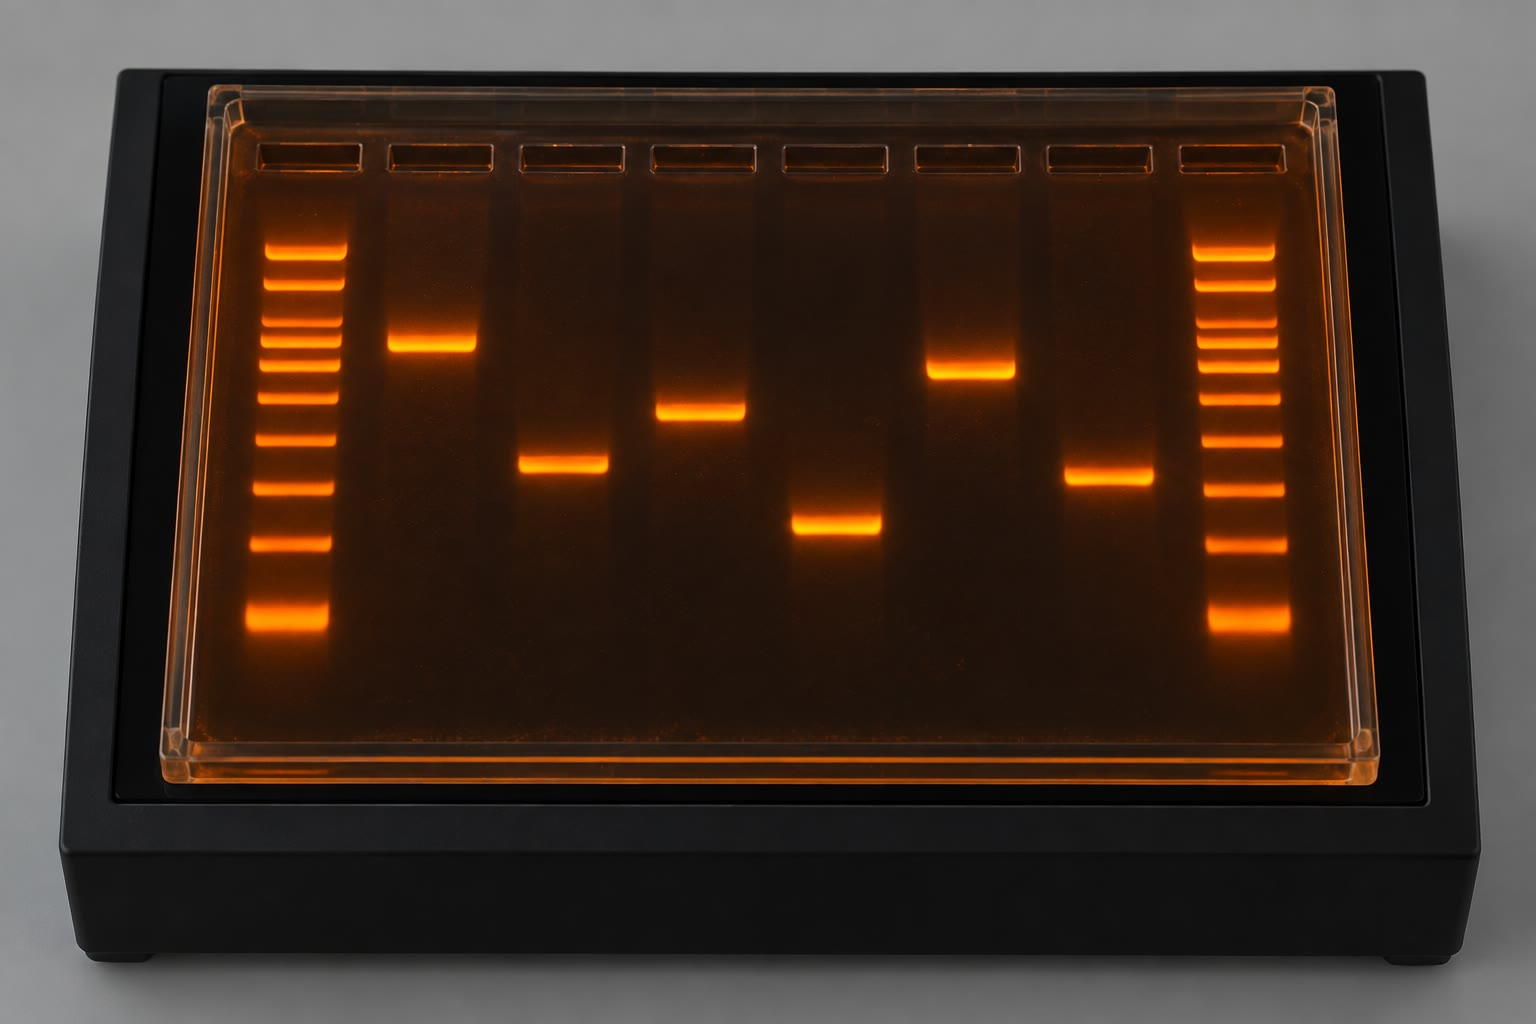
\includegraphics[width=0.56\linewidth]{images/book5/ai/b5-06-agarose-gel.jpg}

{\small 紫外光下的琼脂糖凝胶：DNA 片段向阳极迁移，
迁移速度随片段长度增加而降低，因此每条条带
是同一大小分子的群体，并与外侧泳道中
已知大小的标准梯相比较。}
\end{omfigure}

\begin{definition}[聚合酶链反应]\label{def:b3:genetic-engineering:pcr}
\index{聚合酶链反应}\index{引物}\index{定量 PCR}
\emph{聚合酶链反应}（PCR）在两条\emph{引物}之间扩增选定的
DNA 片段——引物是人工合成的寡核苷酸，长约二十个碱基，
与目标片段两端的两条链互补——经过三种温度的循环：
\qty{95}{\celsius} 使双链分离，
\qtyrange{50}{65}{\celsius} 使引物退火，
\qty{72}{\celsius} 时由耐热聚合酶（Taq，
来自温泉细菌 \emph{Thermus aquaticus}）延伸引物。
每个循环使两引物之间片段的拷贝数翻倍，
因此三十个循环可使单个分子增至十亿个。\emph{逆转录 PCR}
先将 RNA 逆转录为 DNA，因而可检测转录本或 RNA 病毒；
\emph{定量 PCR}（qPCR）借助荧光染料
实时追踪扩增过程，
并由信号越过阈值时所在的循环数
读出起始量。
\end{definition}

\begin{theorem}[扩增的数量关系]\label{thm:b3:genetic-engineering:pcr}
\index{阈值循环数}
设每个循环的效率为 $E$（$E = 1$ 表示完全翻倍），$N_{0}$
个起始拷贝变为
\[
N_{n} = N_{0}\,(1 + E)^{n}
\]
经 $n$ 次循环后，若荧光在
拷贝数达到 $N_{T}$ 时越过固定阈值，则\emph{\omterm{thm:b3:genetic-engineering:pcr}{阈值循环数}}为
\[
C_{T} = \frac{\log N_{T} - \log N_{0}}{\log(1 + E)},
\]
这是关于 $\log N_{0}$ 的直线，斜率为 $-1/\log(1+E)$：对 $E = 1$，
起始量每增加十倍，$C_{T}$ 降低
$\log_{2} 10 = 3.32$ 个循环，两样本的\omterm{thm:b3:genetic-engineering:pcr}{阈值循环数}
相差 $\Delta C_{T}$，二者起始拷贝数之比为
$(1 + E)^{\Delta C_{T}}$。
\end{theorem}
\begin{proof}
每个循环使拷贝数乘以 $1 + E$，因此 $N_{n}$ 是
等比数列。令 $N_{n} = N_{T}$，解出 $n$，得
$C_{T}$；斜率即 $\log N_{0}$ 的系数。对两个样本，
$C_{T,1} - C_{T,2} = (\log N_{0,2} - \log N_{0,1})/\log(1+E)$，由此
可得 $N_{0,2}/N_{0,1} = (1+E)^{\Delta C_{T}}$。
\end{proof}

\begin{example}[读取 qPCR 反应板]\label{ex:b3:genetic-engineering:qpcr}
一次病毒 RNA 检测中，一名患者在第 $22$ 个循环越过阈值，
另一名患者在第 $32$ 个循环越过阈值；取 $E \approx 1$，则前者的病毒量是后者的 $2^{10}
\approx 1000$ 倍。十个拷贝的样本约在
第 $37$ 个循环越过阈值，此时阈值为 $10^{12}$ 拷贝（$\log_{2} 10^{11} =
36.5$）。因此 $40$ 个循环的运行可检出少量分子，而
一个来自前次扩增产物的污染分子同样可被检出，这也是
实验室把配置 PCR 的房间与处理产物的房间
分开的原因。
\end{example}

\begin{omfigure}
\begin{tikzpicture}
\begin{axis}[
  width=0.7\linewidth, height=5.6cm,
  axis x line=bottom, axis y line=left,
  xmin=0, xmax=40, ymin=1, ymax=1e14, ymode=log,
  xlabel={循环数}, ylabel={拷贝数},
  xlabel style={font=\small, at={(axis description cs:0.5,-0.12)}, anchor=north},
  ylabel style={font=\small},
  tick label style={font=\small}, xtick={0,10,20,30,40},
  clip=false,
]
\addplot[very thick, omDef, domain=0:40, samples=41] {1e7*2^x/(1+2^x/1e5)};
\addplot[very thick, omThm, domain=0:40, samples=41] {1e4*2^x/(1+2^x/1e8)};
\addplot[very thick, omMeth!70!black, domain=0:40, samples=41] {10*2^x/(1+2^x/1e11)};
\addplot[dashed, gray, domain=0:40, samples=2] {1e12};
\node[font=\scriptsize, gray, anchor=south west] at (axis cs:0.5,1.3e12) {阈值 $N_{T}$};
\draw[gray] (axis cs:16.6,1) -- (axis cs:16.6,1e12); \draw[gray] (axis cs:26.6,1) -- (axis cs:26.6,1e12); \draw[gray] (axis cs:36.5,1) -- (axis cs:36.5,1e12);
\node[font=\scriptsize, anchor=south] at (axis cs:16.6,3e12) {$C_{T} = 16.6$}; \node[font=\scriptsize, anchor=south] at (axis cs:26.6,3e12) {$26.6$}; \node[font=\scriptsize, anchor=south] at (axis cs:36.5,3e12) {$36.5$};
\end{axis}
\end{tikzpicture}

{\small 扩增曲线：$N_{0} = 10^{7}$（蓝色）、$10^{4}$（红色）
及 $10$ 个拷贝（绿色），$E = 1$，并标出试剂所限定的平台。
$N_{0}$ 相差千倍时，\omterm{thm:b3:genetic-engineering:pcr}{阈值循环数}改变 $10$；各条曲线的平台都相同，
这正是终产物无法说明起始量的原因。}
\end{omfigure}

\section{制备蛋白质}

\begin{definition}[表达系统]\label{def:b3:genetic-engineering:expression}
\index{表达载体}\index{重组蛋白}\index{单克隆抗体}
\emph{表达\omterm{def:b3:genetic-engineering:tools}{载体}}将所克隆的编码序列置于宿主的一个强而可控的
启动子之下（\emph{lac} 或 T7
启动子，在 \emph{E.~coli} 中由糖类类似物诱导），
并带有核糖体结合位点、终止子，还常加一个\emph{标签}——
六个组氨酸，即一小段蛋白，与产物融合，以便在柱上
纯化。细菌每升可产数克简单的蛋白质
（如胰岛素、生长激素、酶），却不能糖基化，也不能折叠
复杂的哺乳动物蛋白；酵母则加上其特有类型的糖类；昆虫
与哺乳动物细胞（中国仓鼠卵巢细胞是行业标准）
能制造与人体内一样折叠、糖基化的抗体和凝血因子。
\emph{单克隆抗体}可由
\emph{杂交瘤}制得——即将产抗体的 B 细胞与永生骨髓瘤细胞融合
（科勒与米尔斯坦，1975）——或如今将
抗体基因导入哺乳动物表达细胞株，其中小鼠框架区可替换为人源序列，
以避免免疫排斥
（见\cref{ch:b3:adaptive-immunity}）。
\end{definition}

\begin{example}[胰岛素]\label{ex:b3:genetic-engineering:insulin}
人胰岛素由两条链组成：A 链含 21 个残基，B 链含 30 个残基，
两链以二硫键相连，在 $\beta$ 细胞中由单一胰岛素原前体切割而成。
第一种工艺是把两条链分别在
\emph{E.~coli} 中表达，每条链都与 $\beta$-半乳糖苷酶融合，
之后用化学方法切下，并在体外将两条链连接起来；后来的工艺则直接表达胰岛素原，
再用胰腺所用的酶将其切割。自 1996 年以来，
序列本身已被改造：替换或增加一两个残基，
便得到解离更快（用于进餐时）或在注射
部位沉淀并在一天内释放的类似物。一种蛋白曾经每千克需八
吨腺体，如今在发酵罐中生产，
与人体蛋白相同，甚至更优。
\end{example}

\section{转基因生物}

\begin{definition}[转基因技术与基因打靶]\label{def:b3:genetic-engineering:transgenic}
\index{转基因生物}\index{显微注射}\index{敲除}\index{胚胎干细胞}\index{基因打靶}
\emph{转基因}生物的生殖系中携带一个导入的基因，
使每个细胞都含有该基因，并可遗传。在小鼠中，经典方法是
将 DNA \emph{显微注射}到
受精卵的一个原核中（戈登和拉德尔，1980），注入的 DNA 随机整合
于一部分胚胎的某一位点；帕尔米特和布林斯特（1982）
通过注入置于金属硫蛋白启动子之后的大鼠生长激素基因，
使小鼠体型达到正常的两倍。\emph{基因打靶}则是替换或破坏
某个指定基因：将一个两侧带有与靶位点同源长臂的重组构建体
导入\emph{胚胎干细胞}，其中罕见的细胞里，\omterm{def:b3:dna-repair:dsb}{同源重组}恰好将其
置于正确位置的细胞被筛选出来，
再注入囊胚，所得的嵌合小鼠
能够将改造后的基因传给后代（卡佩基、史密瑟斯和埃文斯，
1980 年代）。\emph{敲除}是指缺失该基因；\emph{敲入}是指携带
经修饰的版本；\emph{条件性}等位基因两侧带有 loxP 位点，
仅在 Cre 表达的部位和时间才被删除
（见\cref{ch:b3:dna-repair}）。约一万个小鼠基因
已被敲除，对大多数基因而言，表型往往是
人们首次了解其功能的线索。
\end{definition}

\begin{omfigure}
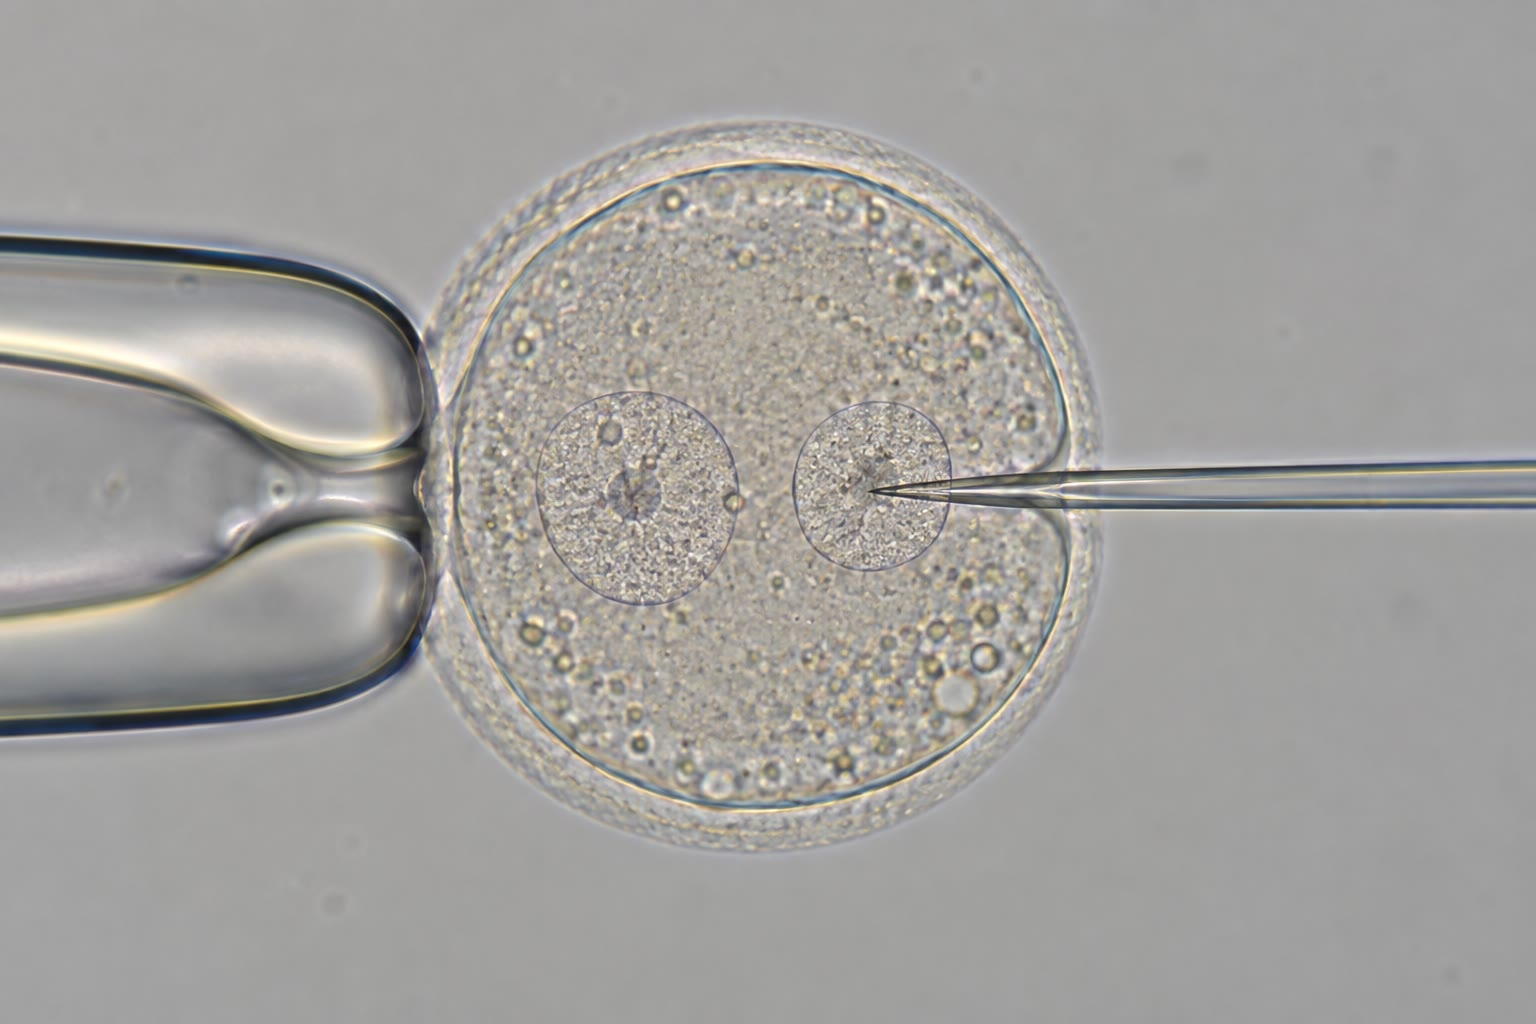
\includegraphics[width=0.46\linewidth]{images/book5/ai/b5-06-microinjection.jpg}\hspace{0.04\linewidth}
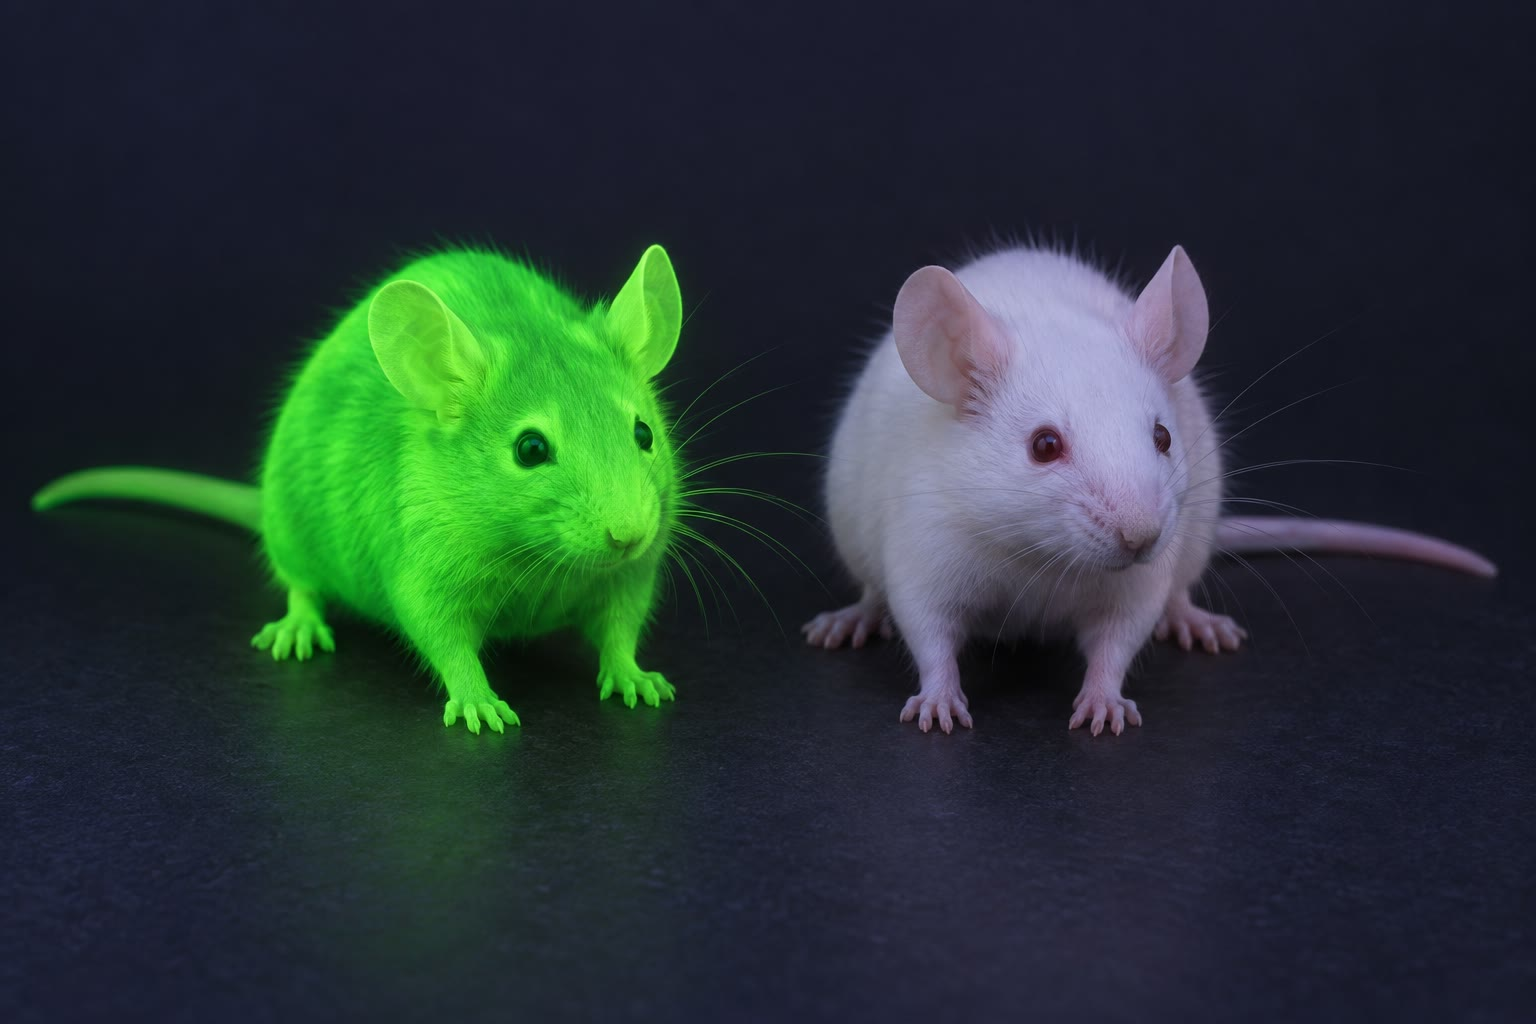
\includegraphics[width=0.46\linewidth]{images/book5/ai/b5-06-gfp-mouse.jpg}

{\small 左：一枚受精小鼠卵被吸管固定，玻璃针将 DNA 注入其一个原核。
右：一只\omterm{def:b3:genetic-engineering:transgenic}{转基因}小鼠，
在每个细胞中表达水母的绿色荧光蛋白，
与一只普通同窝小鼠并排，置于紫外线下。}
\end{omfigure}

\begin{definition}[转基因植物]\label{def:b3:genetic-engineering:plants}
\index{Agrobacterium}\index{T-DNA}\index{转基因作物}
植物通过 \emph{Agrobacterium tumefaciens} 转化。该菌是一种土壤细菌，
能自然地将自身肿瘤诱导\omterm{def:b3:genetic-engineering:tools}{质粒}的一段（即
\emph{T-DNA}）插入受伤植物的基因组，使其长出瘤状组织，
并为细菌提供养分。把 T-DNA 自身的基因
替换为任意所需基因，置于细菌所识别的边界序列之间，
使这一病原体成为\omterm{def:b3:genetic-engineering:tools}{载体}；被转化的细胞
经筛选后再生为完整植株，这是每个植物细胞
都能做到的。细菌不能感染的物种（谷类作物，
长期以来如此）则通过将包裹 DNA 的金颗粒射入
组织来完成转化。大规模种植的\emph{\omterm{def:b3:genetic-engineering:transgenic}{转基因}作物}携带
一个细菌毒素基因（\emph{Bt}）以抵御昆虫幼虫，或携带
一个赋予除草剂耐受性的细菌酶基因，或两者兼有；\emph{黄金大米}
带有类胡萝卜素途径中的两个基因（一个植物八氢番茄红素合酶基因
和一个细菌去饱和酶基因），使其胚乳能够合成
$\beta$-胡萝卜素，即维生素~A 的前体，其缺乏
每年导致数十万名儿童失明和死亡。
\end{definition}

\begin{omfigure}
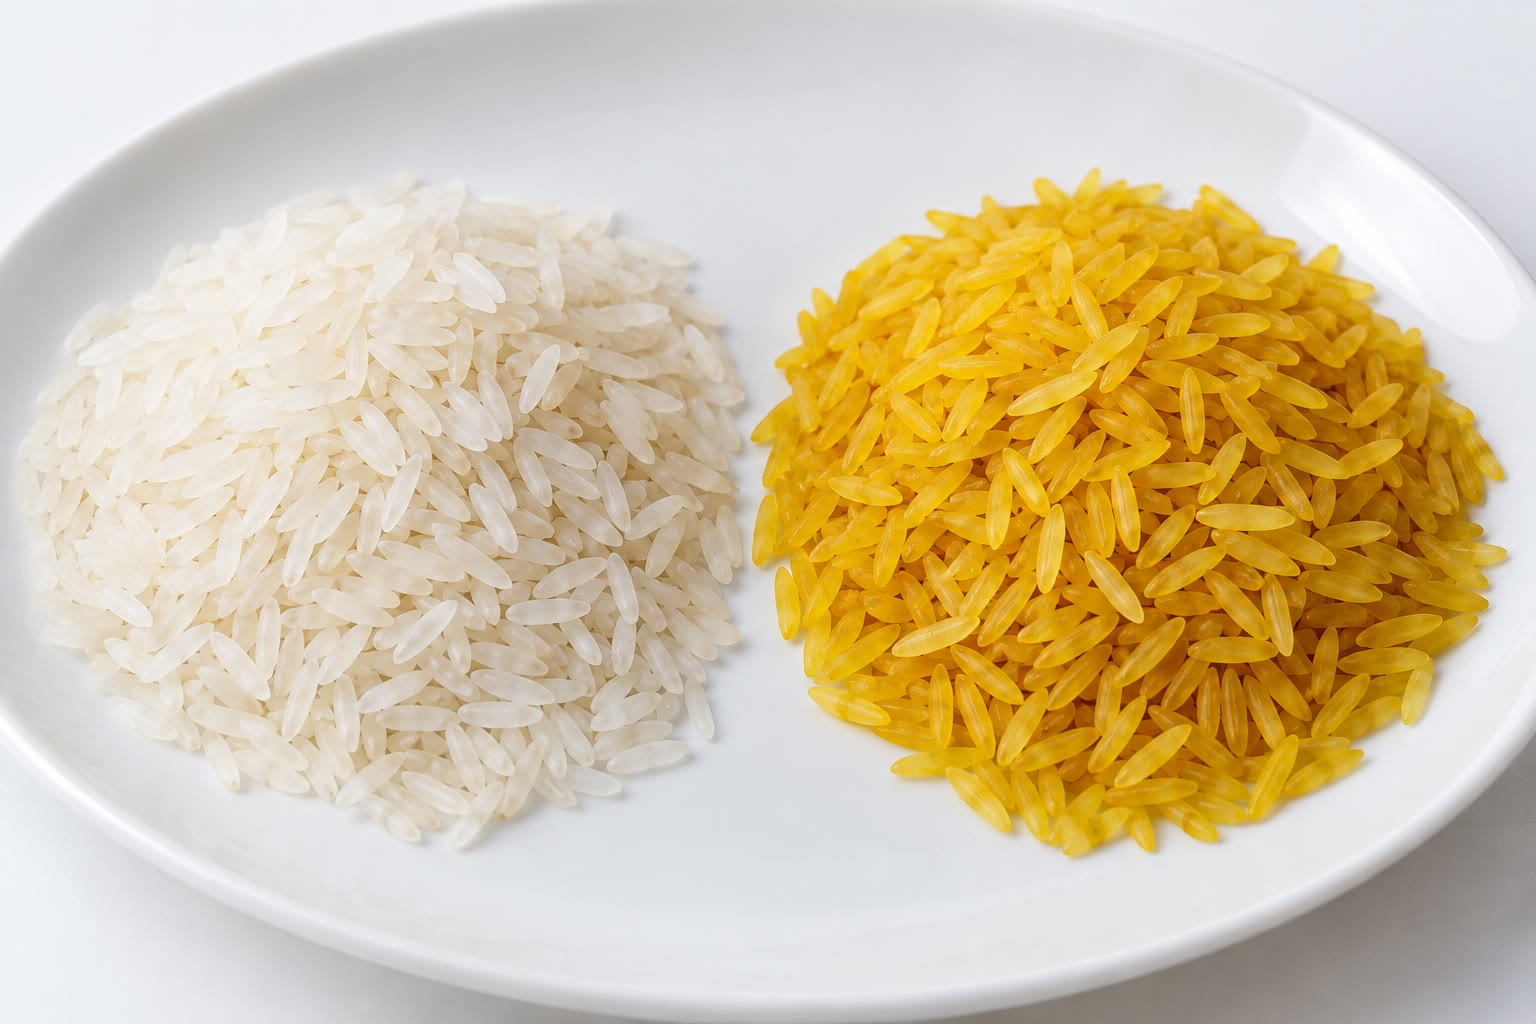
\includegraphics[width=0.46\linewidth]{images/book5/ai/b5-06-golden-rice.jpg}\hspace{0.04\linewidth}
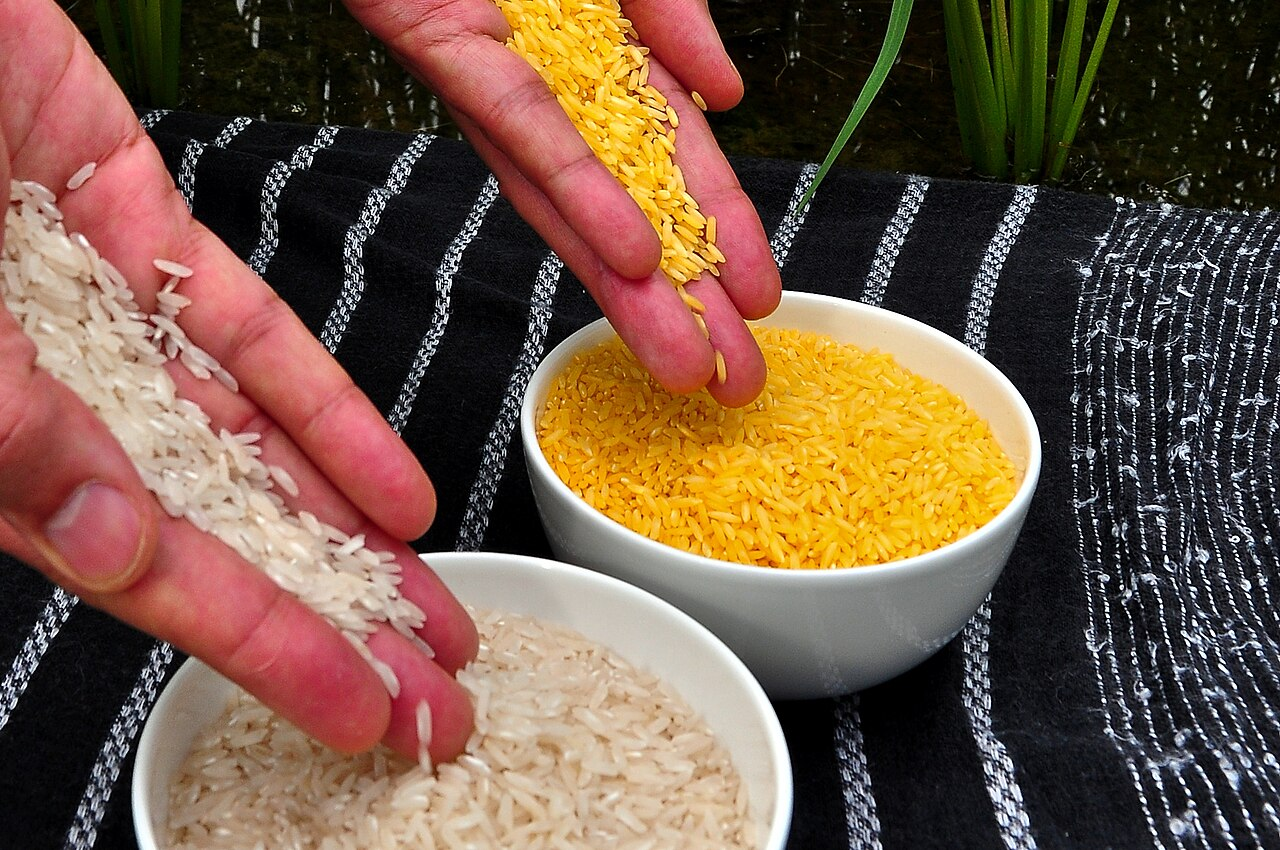
\includegraphics[width=0.46\linewidth]{images/book5/golden-rice-irri.jpg}

{\small 普通水稻与黄金大米。黄色籽粒的胚乳中，
由两个外加的类胡萝卜素途径基因合成 $\beta$-胡萝卜素。
右：两种水稻在
国际水稻研究所（IRRI，CC~BY~2.0）进行比较。}
\end{omfigure}

\begin{remark}[争论]\label{rem:b3:genetic-engineering:gmo}
三十年来，数亿公顷土地上种植了获批的\omterm{def:b3:genetic-engineering:plants}{转基因作物}，
各国科学院的每一项系统综述均未发现，这些作物
有任何与常规作物不同的健康效应；
\omterm{def:b3:genetic-engineering:transgenic}{转基因}只是约四万个基因中的又一个，
其所产蛋白质与任何食品添加剂一样接受检验。
真正的问题是生态与经济方面的：
在统一选择压力下，害虫和杂草的抗性扩散，基因流入
野生近缘种，种子市场的集中，以及
利益归于谁。这些问题是任何具有重大影响的
农业技术都会提出的，其答案取决于性状和环境，
而与基因的导入方式无关。
\end{remark}

\section{基因组编辑}

\begin{definition}[CRISPR--Cas9]\label{def:b3:genetic-engineering:crispr}
\index{CRISPR}\index{Cas9}\index{向导 RNA}\index{PAM}\index{基因组编辑}
细菌将感染过其祖先的噬菌体的基因组片段
保存在一段重复序列阵列（\emph{CRISPR}）中，将其转录为
短向导 RNA，并用它们引导核酸酶切割进入细胞的任何
匹配的 DNA：这是一种具有遗传记忆的适应性免疫系统。
在 \emph{Streptococcus pyogenes} 中，核酸酶是
单一蛋白质 \emph{Cas9}，它结合一条向导 RNA 和另一条小
RNA，在 DNA 中寻找一个三碱基的\emph{原间隔序列邻近\omterm{def:b3:bioinformatics:motif}{基序}}
（PAM，5$'$-NGG），解开邻近的 DNA；若与 PAM 相邻的二十个碱基
与向导配对，则在距 PAM 三个碱基处
切断两条链。金内克、夏彭蒂耶、杜德纳等人（2012）将两条
RNA 融合为一条\emph{单向导 RNA}，并证明带有
任意所选序列向导的 Cas9 能在试管中于该序列处切割 DNA；
一年之内，这一组合已被证明可在人、小鼠、斑马鱼、
植物和酵母细胞中发挥作用。\emph{基因组编辑}是指细胞
对切口的处理：末端连接会留下一个小的插入或缺失，
从而破坏基因（一步即可得到\omterm{def:b3:genetic-engineering:transgenic}{敲除}，适用于任何生物，只需数周）；
而借助提供的模板进行\omterm{def:b3:dna-repair:dsb}{同源重组}，可写入一段
指定序列。
\end{definition}

\begin{omfigure}
\begin{tikzpicture}[every node/.style={font=\scriptsize}, >=stealth]
  % Cas9 outline (drawn first so labels stay on top)
  \draw[thick, omExo, fill=omExo!15] (5.9,1.1) ellipse (2.6 and 1.6);
  \node[omExo!60!black] at (7.7,2.3) {Cas9 蛋白};
  % target DNA
  \draw[very thick, omDef] (0,0.3) -- (11,0.3); \draw[very thick, omDef] (0,-0.1) -- (11,-0.1);
  % PAM
  \fill[omProp!60] (7.2,-0.2) rectangle (7.9,0.4); \node[below] at (7.55,-0.25) {PAM（NGG）};
  % protospacer
  \draw[omThm, very thick] (4.2,0.5) -- (7.15,0.5); \node[above] at (5.7,0.55) {20 个碱基的靶点，与向导配对};
  % guide RNA
  \draw[very thick, omMeth!70!black] (4.2,0.3) .. controls (4.2,1.6) and (5.0,1.9) .. (5.4,1.9) -- (6.6,1.9) .. controls (7.0,1.9) and (7.2,2.5) .. (6.8,2.8) .. controls (6.3,3.1) and (5.8,2.7) .. (6.1,2.4);
  \node[left, omMeth!70!black, align=right] at (3.2,2.2) {单向导 RNA：\\任选 20 个碱基 \\+ Cas9 结合发夹};
  % cut
  \draw[omThm, very thick, ->] (6.25,-0.7) -- (6.25,0.35); \node[omThm, below] at (6.25,-0.7) {双链断裂，距 PAM 3 个碱基};
  % outcomes
  \draw[->, thick] (2.0,-1.3) -- (2.0,-1.9); \node[below, align=center] at (2.0,-1.9) {末端连接：\\小的插入或缺失 \\$\Rightarrow$ 移码，敲除};
  \draw[->, thick] (10.0,-1.3) -- (10.0,-1.9); \node[below, align=center] at (10.0,-1.9) {与提供模板的重组 \\$\Rightarrow$ 精确改变};
\end{tikzpicture}

{\small \omterm{def:b3:genetic-engineering:crispr}{Cas9} 与其向导。该蛋白结合 \omterm{def:b3:genetic-engineering:crispr}{PAM}，在其旁解开 DNA
双链，若二十个碱基与向导 RNA 配对，则切割。
断裂处可通过末端连接修复，这会破坏基因，或
经与模板的重组修复，这会改写基因。}
\end{omfigure}

\begin{proposition}[无断裂编辑]\label{prop:b3:genetic-engineering:editors}
\index{碱基编辑器}\index{先导编辑器}\index{脱靶}
切断两条链是最粗糙的编辑：末端连接的结果是
随机的，而在别处的断裂——一个\emph{\omterm{prop:b3:genetic-engineering:editors}{脱靶}}位点，
与向导仅在少数位置不同，而 \omterm{def:b3:genetic-engineering:crispr}{Cas9} 能够容忍这种差异——是一种
无人所求的突变。带有一个核酸酶结构域失活的 \omterm{def:b3:genetic-engineering:crispr}{Cas9}
切开一条单链；两个结构域均失活时，它仅能结合，并可
将其他酶带至某一序列。\emph{\omterm{prop:b3:genetic-engineering:editors}{碱基编辑器}}将切口型 \omterm{def:b3:genetic-engineering:crispr}{Cas9} 与一种
脱氨酶融合，该酶可在解开的链上将 C 转化为 U（读作 T），或将 A 转化为 I
（读作 G），从而在不断裂、也不用模板的情况下改变一个碱基；
\emph{\omterm{prop:b3:genetic-engineering:editors}{先导编辑器}}携带一种逆转录酶，并
以一条延伸出所需序列的向导，将该序列复制到切口链上，
从而允许任意替换以及小片段的插入或缺失。\omterm{prop:b3:genetic-engineering:editors}{脱靶}活性可
通过工程化的高保真 \omterm{def:b3:genetic-engineering:crispr}{Cas9} 变体降低，
也可通过以蛋白形式而非基因形式短暂递送该酶来降低，
或选择其最近基因组同源序列在多个位置存在差异的向导来降低；
其检测方法为对预测位点进行测序，并
采用无偏方法捕获
基因组中的每一次断裂。
\end{proposition}

\begin{example}[一种治愈]\label{ex:b3:genetic-engineering:sickle}
镰状细胞病是 $\beta$-珠蛋白中的单个碱基改变。胎儿
血红蛋白由 $\gamma$-珠蛋白构成，本可替代，但
$\gamma$ 基因在出生后被阻遏蛋白 BCL11A 关闭。
首个获批的 \omterm{def:b3:genetic-engineering:crispr}{CRISPR} 疗法（2023 年）取患者自身的造血干细胞，
用 \omterm{def:b3:genetic-engineering:crispr}{Cas9} 切割 \emph{BCL11A} 的红系增强子，使多数细胞中的末端连接令其失活，
待患者骨髓清除后将细胞回输。
由此生成的红细胞富含胎儿血红蛋白，
不再镰变，危象也随之停止。该编辑属于体细胞编辑，
生殖系未受影响，改变也不会遗传；它利用的是
“粗糙”的结果，即破坏，而在此处
所需的正是破坏。
\end{example}

\begin{theorem}[基因驱动的超孟德尔式扩散]\label{thm:b3:genetic-engineering:drive}
\index{基因驱动}
\emph{\omterm{thm:b3:genetic-engineering:drive}{基因驱动}}是一种携带 \omterm{def:b3:genetic-engineering:crispr}{Cas9} 及向导的构建体，它在杂合子中切割
其自身基因座上的野生型等位基因；经重组修复，
驱动元件被复制到被切断的染色体上，因此
杂合子中比例为 $c$ 的配子携带驱动元件，而非
孟德尔的一半。设驱动元件的频率为 $p$，
处于大型随机交配种群中，且无适合度代价，
则其在下一代的频率为
\[
p' = p + c\,p\,(1 - p),
\]
因此它自稀少状态起，以正比于 $c$ 的速率扩散，并
达到种群一半所需的代数约为 $\ln(1/p_{0})/\ln(1 + c)$，
自初始频率 $p_{0}$ 出发。
\end{theorem}
\begin{proof}
随机交配下，驱动纯合子的频率为 $p^{2}$，
杂合子的频率为 $2p(1-p)$，野生型纯合子的频率为 $(1-p)^{2}$。
驱动纯合子将驱动元件传给其全部配子，杂合子则
以比例 $(1 + c)/2$ 传递驱动元件（孟德尔的一半，加上野生型一半中
被转换的 $c$ 倍），野生型纯合子则不传递。由此 $p' = p^{2} + 2p(1-p)(1+c)/2
= p^{2} + p(1-p) + c\,p(1-p) = p + c\,p(1-p)$。当 $p$ 较小时，此式为
$p' \approx (1+c)p$，即以公比 $1 + c$ 的几何增长，
达到 $1/2$（自 $p_{0}$ 出发）约需 $\ln(1/2p_{0})/\ln(1+c)$ 代；
逻辑斯谛项只在接近终点时才减缓其增长。
\end{proof}

\begin{omfigure}
\begin{tikzpicture}
\begin{axis}[
  width=0.7\linewidth, height=5.6cm,
  axis x line=bottom, axis y line=left,
  xmin=0, xmax=20, ymin=0, ymax=1.05,
  xlabel={代数}, ylabel={驱动频率 $p$},
  xlabel style={font=\small, at={(axis description cs:0.5,-0.12)}, anchor=north},
  ylabel style={font=\small},
  tick label style={font=\small}, xtick={0,5,10,15,20}, ytick={0,0.5,1},
  clip=false,
]
\addplot[very thick, omThm, mark=*, mark size=1.2pt] coordinates {(0,0.01) (1,0.0189) (2,0.0356) (3,0.0665) (4,0.1224) (5,0.2191) (6,0.3731) (7,0.5836) (8,0.8023) (9,0.9451) (10,0.9918) (11,0.9991) (12,1.0) (13,1.0) (14,1.0) (15,1.0) (16,1.0) (17,1.0) (18,1.0) (19,1.0) (20,1.0)};
\addplot[very thick, omDef, mark=*, mark size=1.2pt] coordinates {(0,0.01) (1,0.015) (2,0.0223) (3,0.0332) (4,0.0493) (5,0.0727) (6,0.1064) (7,0.154) (8,0.2191) (9,0.3047) (10,0.4106) (11,0.5316) (12,0.6561) (13,0.769) (14,0.8578) (15,0.9188) (16,0.9561) (17,0.9771) (18,0.9883) (19,0.9941) (20,0.997)};
\addplot[very thick, gray, dashed, domain=0:20, samples=2] {0.01};
\node[font=\scriptsize, omThm, anchor=south east] at (axis cs:6.5,0.62) {$c = 0.9$};
\node[font=\scriptsize, omDef, anchor=north west] at (axis cs:12.5,0.62) {$c = 0.5$};
\node[font=\scriptsize, gray, anchor=south west] at (axis cs:12,0.02) {孟德尔式，$c = 0$：保持在 $p_{0}$};
\end{axis}
\end{tikzpicture}

{\small \omterm{thm:b3:genetic-engineering:drive}{基因驱动}以百分之一的频率释放，转化效率分别为
$0.9$ 或 $0.5$，且无适合度代价。无优势的孟德尔式等位基因
将保持在百分之一；驱动元件在十或
二十代内取而代之。}
\end{omfigure}

\begin{remark}[可以编辑什么]\label{rem:b3:genetic-engineering:ethics}
对知情同意的患者的体细胞进行编辑，属于医疗行为，
与任何治疗一样依其风险和获益加以判断。而编辑生殖系——
即一枚胚胎，其所有后代都将携带该改变——
性质上迥然不同：受影响者无法表示同意，该改变
会遗传，且该技术的\omterm{prop:b3:genetic-engineering:editors}{脱靶}与嵌合结果尚未得到控制；
此前，一位中国科学家于 2018 年宣布，他已
对双胞胎做了此操作。多数国家的科学院呼吁
暂停相关研究，并有数个国家将其定为犯罪。\omterm{thm:b3:genetic-engineering:drive}{基因驱动}
若释放到野生种群中，便是替所有人作出的决定，
其影响将及于下游，这正是该领域自身提出的消除
疟蚊方案要将驱动与故障安全机制相结合——例如逆转驱动，
自限设计——并以
相关国家的公众同意为前提。
\end{remark}

\section{练习}

\begin{exercise}[$\star$]\label{exo:b3:genetic-engineering:1}
列出克隆\omterm{def:b3:genetic-engineering:tools}{质粒}必须具备的三个组成部分，并
说明各自的作用。
\end{exercise}

\begin{exercise}[$\star$]\label{exo:b3:genetic-engineering:2}
EcoRI 识别 GAATTC。该位点在随机 DNA 中平均多久出现一次，
以及它会把 \qty{4.6}{Mb} 的
\emph{E.~coli} 基因组切成多少个片段？为什么实际数目与此略有不同？
\end{exercise}

\begin{exercise}[$\star$]\label{exo:b3:genetic-engineering:3}
说出 PCR 一个循环的三个温度步骤，以及
每一步发生的过程。为什么聚合酶必须耐热？
\end{exercise}

\begin{exercise}[$\star$]\label{exo:b3:genetic-engineering:4}
\omterm{def:b3:genetic-engineering:crispr}{Cas9} 切割某一给定序列需要什么条件，以及
切割之后可能出现哪两种结果？
\end{exercise}

\begin{exercise}[$\star\star$]\label{exo:b3:genetic-engineering:5}
一次 PCR 进行 $35$ 个循环，效率 $E = 0.9$，
起始为 $50$ 个拷贝，最终得到多少个拷贝？对两个样品做 qPCR，得到 $C_{T} = 18.2$ 和 $25.5$；
取 $E = 0.95$，求二者起始量之比。
\end{exercise}

\begin{exercise}[$\star\star$]\label{exo:b3:genetic-engineering:6}
为什么在细菌中表达人源蛋白时，使用的是 cDNA \omterm{met:b3:genetic-engineering:cloning}{文库}而不是
基因组\omterm{met:b3:genetic-engineering:cloning}{文库}？请再说出制备人源蛋白的另外两个障碍，
以 \emph{E.~coli} 为宿主，并说明各自如何克服。
\end{exercise}

\begin{exercise}[$\star\star$]\label{exo:b3:genetic-engineering:7}
通过\omterm{def:b3:genetic-engineering:transgenic}{胚胎干细胞}的\omterm{def:b3:genetic-engineering:transgenic}{基因打靶}制备\omterm{def:b3:genetic-engineering:transgenic}{敲除}小鼠。
试说明：为什么最初出生的小鼠是嵌合体，为什么必须让它繁殖？
并求出一只生殖系有一半被打靶的嵌合体，其孙代中
纯合\omterm{def:b3:genetic-engineering:transgenic}{敲除}个体所占的比例是多少，前提是杂合的祖父母
相互交配。
\end{exercise}

\begin{exercise}[$\star\star$]\label{exo:b3:genetic-engineering:8}
选取一条 20 个碱基、带 NGG \omterm{def:b3:genetic-engineering:crispr}{PAM} 的向导 RNA。在
$3.2\times 10^{9}$ bp 的基因组（双链计）中，偶然与该向导完全匹配的位点有多少个？
若 \omterm{def:b3:genetic-engineering:crispr}{Cas9} 可容忍这些错配，则允许至多两个错配的位点有多少个？
（错配数不超过两个的序列计为 $1 + 3\binom{20}{1} +
9\binom{20}{2}$。）
\end{exercise}

\begin{exercise}[$\star\star$]\label{exo:b3:genetic-engineering:9}
利用\cref{thm:b3:genetic-engineering:drive}，计算
$c = 0.8$ 的驱动，从 $p_{0} = 0.05$ 出发，经过三代后的
频率，并估计达到 $0.5$ 所需的代数。
\end{exercise}

\begin{exercise}[$\star\star\star$]\label{exo:b3:genetic-engineering:10}
镰刀型细胞贫血症的疗法是破坏一个增强子，而不是
纠正 $\beta$-珠蛋白突变。试给出两个理由，说明为何
在造血干细胞中选择末端连接破坏，而不是\omterm{def:b3:dna-repair:dsb}{同源重组}纠正，
并给出一个缺点。
\end{exercise}

\begin{exercise}[$\star\star\star$]\label{exo:b3:genetic-engineering:11}
针对蚊子的一种\omterm{thm:b3:genetic-engineering:drive}{基因驱动}在纯合子中携带适合度代价 $s$，
修改递推关系，使其包含对驱动纯合子的选择，
并求出驱动从稀少状态开始扩散所需的 $c$ 与 $s$ 之间的条件。
随后解释：为什么抗性等位基因——靶位点上经末端连接
产生、向导不再识别的产物——是实践中的
主要障碍。
\end{exercise}

\begin{exercise}[$\star\star\star$]\label{exo:b3:genetic-engineering:12}
结合本章及
\cref{ch:b3:dna-repair}中的机制，论证为什么目前对人类胚胎进行生殖系编辑，
无法保证每个细胞都获得预期结果，并说明
理性的人在考虑其安全性之前，需要哪些
证据。
\end{exercise}

\section{问题：从基因到药物与作物}

\begin{problem}[{周末问题——借助限制性位点与转化的计算克隆一个基因，
用 qPCR 计数一种病毒，计算发酵罐中以吨计的激素产量，
统计编辑后基因组的脱靶位点，
为一个基因驱动计时，最后以样品中病毒的拷贝数、
全世界胰岛素所需的年发酵罐体积
以及驱动所需的代数}]
\label{pb:b3:genetic-engineering:1}
数据：一个 \qty{1.5}{kb} 的基因；一个六碱基的限制性位点；一个
\qty{4}{kb} 的\omterm{def:b3:genetic-engineering:tools}{质粒}；转化效率为 $2\times 10^{7}$ 个菌落每
微克\omterm{def:b3:genetic-engineering:tools}{质粒}；连接反应使 \qty{10}{\%} 的\omterm{def:b3:genetic-engineering:tools}{质粒}获得
插入片段。qPCR 效率 $E = 1$，阈值 $N_{T} = 10^{12}$。胰岛素：
\qty{5.8}{kDa}，患者每天用 $40$ 个单位，每个单位为
\qty{35}{\micro g}；$10^{7}$ 名患者；发酵罐每批次产出
\qty{2}{g/L} 的产物，每年 10 批。基因组 $3.2\times
10^{9}$ bp。驱动转化率 $c = 0.9$，以 $p_{0} = 0.001$ 释放。

\medskip
\noindent\textbf{第一部分——克隆。}
\begin{enumerate}
  \item 某一六碱基位点在随机 DNA 中平均多久出现一次？
        \qty{1.5}{kb} 的基因中不含此类位点的概率是多少，
        从而可用该酶将其完整克隆？
  \item 若该基因中确有此类位点，仍要克隆它，应如何操作？
        （两种方法。）
  \item 对 \qty{100}{ng} 的连接后\omterm{def:b3:genetic-engineering:tools}{质粒}进行转化，
        可得多少个菌落，其中多少个携带插入片段？
  \item 采用蓝白筛选，白色菌落占全部菌落的比例是多少，
        以及需挑选多少个白色菌落，才能使其中至少一个
        携带正确取向基因的概率达到 \qty{99}{\%}
        （插入片段中取向正确者占一半）？
  \item 重组\omterm{def:b3:genetic-engineering:tools}{质粒}为 \qty{5.5}{kb}。一个细胞含有 $50$
        个拷贝，每 \qty{30}{min} 分裂一次。从单个细胞开始
        过夜生长（\qty{16}{h}）后，共有多少个\omterm{def:b3:genetic-engineering:tools}{质粒}分子，
        以及\omterm{def:b3:genetic-engineering:tools}{质粒} DNA 的质量是多少（每碱基对 \qty{650}{Da}）？
  \item 为什么\omterm{def:b3:genetic-engineering:tools}{质粒}需要细菌复制起点，而插入的人源基因
        在克隆时不需要细菌启动子，而在表达时
        则需要启动子？
\end{enumerate}

\medskip
\noindent\textbf{第二部分——病毒计数。}
\begin{enumerate}[resume]
  \item 某患者样本在 $C_{T} = 28$ 时越过阈值，
        反应中有多少个拷贝？另一样本的 $C_{T} = 35$ 又是多少？
  \item 灵敏度：需要多少个循环，才能使单个拷贝
        扩增至阈值？
  \item 检测的截断值设为 $C_{T} = 38$，该值对应多少个拷贝，
        以及为何不用 $45$ 个循环？
  \item 上一次反应的产物中的一个污染分子进入了一个
        阴性样本。它在第几个循环越过阈值？
        哪种实验室操作可以防止这种情况？
  \item 逆转录可将病毒 RNA 的 \qty{40}{\%} 转化为
        DNA。请对第一个样本校正第~7~题中的拷贝数。
  \item 两样本的 $\Delta C_{T} = 3.3$，按 $E = 1$ 计算，但
        实际效率为 $0.9$。分析人员报告的倍数差异是多少，
        真实的倍数差异又是多少？
\end{enumerate}

\medskip
\noindent\textbf{第三部分——胰岛素的吨级生产。}
\begin{enumerate}[resume]
  \item 计算每位患者每日所需的胰岛素质量，以及
        $10^{7}$ 名患者全年所需的全球胰岛素质量（以千克计）。
  \item 这些胰岛素相当于多少摩尔，含有多少个分子？
  \item 若每年运行十批次，需要多大体积的发酵罐才能生产这些胰岛素？
        与一个 \qty{2500}{m^3} 的游泳池相比较。
  \item 从腺体提取时，得到 \qty{1}{kg} 胰岛素需用
        \qty{8000}{kg} 胰腺；一头猪的胰腺重 \qty{100}{g}。
        全球每年需要多少头猪？
  \item 即使在动物胰岛素价格低廉的地方，为何仍优先选用
        重组激素？请给出两个理由。
  \item 胰岛素类似物与人源序列相差一个或两个
        残基。请解释为何类似物仍是作用于
        人受体的药物，以及为何一个残基的改变会改变
        其解离时间。
\end{enumerate}

\medskip
\noindent\textbf{第四部分——编辑与驱动。}
\begin{enumerate}[resume]
  \item 基因组中偶然出现的、与 20 个碱基的向导加 NGG
        完全匹配的位点有多少个（两条链共 $6.4\times 10^{9}$
        个位置）？
  \item 若 \omterm{def:b3:genetic-engineering:crispr}{Cas9} 可容忍至多三个错配，则与向导序列
        错配不超过三个的序列有多少个，由此产生多少个偶然
        \omterm{prop:b3:genetic-engineering:editors}{脱靶}位点？
  \item 经编辑的造血干细胞共 $10^{7}$ 个，其中 \qty{80}{\%} 带有
        预期的破坏。有多少个细胞在某一位点携带\omterm{prop:b3:genetic-engineering:editors}{脱靶}
        断裂（若该位点每 $10^{4}$ 个细胞中有一个被切割），
        以及为何单个干细胞中抑癌基因的断裂
        值得关注？
  \item 计算驱动等位基因在 $1, 2, 3$ 代后的频率，初始值为
        $p_{0} = 0.001$，并估算达到 $0.5$ 所需的代数。
  \item 蚊子每年繁衍十代。驱动等位基因需要多少年才能
        占据群体？纯合子中 \qty{20}{\%} 的适合度代价会如何
        从定性角度改变这一情形？
  \item 当切割由末端连接而非重组修复时，会产生抗性等位基因，
        每次转化尝试中修复切口的概率为 $1 - c = 0.1$。
        估算一代中在 $10^{6}$ 个杂合子群体内产生的
        抗性等位基因数，
        并说明若这些等位基因具有适合度，驱动会发生什么变化。
  \item 汇总以下内容：第一个样本中的拷贝数（第~7~题），
        全球每年胰岛素发酵罐体积（第~15~题），以及
        驱动等位基因达到半数群体所需的代数
        （第~22~题）。
\end{enumerate}
\end{problem}
